\documentclass[12pt,a4paper]{article}

\usepackage[utf8]{inputenc}
\usepackage[english]{babel}
\usepackage{amsmath}
\usepackage{amsfonts}
\usepackage{amssymb}
\usepackage{makeidx}
\usepackage{graphicx}
\usepackage{subcaption}
\usepackage{caption}
\usepackage{float}
\usepackage[left=2cm,right=2cm,top=2cm,bottom=2cm]{geometry}
\usepackage{tikz}
\usepackage{pdfpages}
\pagestyle{plain}
\usepackage{bm}
\usepackage{ulem}
\usepackage{units}
\usepackage{makecell}

%Kopf und Fußzeile:
\usepackage{fancyhdr}
\pagestyle{fancy}
\fancyhf{}
\renewcommand{\footrulewidth}{0.4pt}
\usepackage{array}   % for \newcolumntype macro
\newcolumntype{C}{>{$}c<{$}} % math-mode version of "c" column type

\fancyhead[L]{Computational photonics}
%\fancyhead[C]{Dr. Bj\"orn Leder}
\fancyhead[R]{Excercise 2}
\fancyfoot[L]{\today}
\fancyfoot[R]{page \thepage}
\fancyfoot[C]{Julien Kluge}

% Code-Listings
\usepackage{listings}
\lstset{
language=c,
showstringspaces=false,
numbers=left,
xleftmargin=2em}

% Ganze Dateien als Verbatim einbinden
%\usepackage{verbatimfiles} % downloaded from ctan.org

\title{Computational photonics}
\author{Julien Kluge}
\date{\today}

%============================================================
% Dokument
%============================================================
\begin{document}

\lstset{numbers=left}

\begin{center}
\large{\textbf{Computational photonics -- Excercise 2}} \\
~\\
\small{-- Julien Kluge (564513) --}\\
~\\
Date: \today
\end{center}
\hrule

\section*{Preliminary quote}
	\textit{Well, I had an amazing and exciting week in the lab. Sooo, I neglected the excercise a bit.
	I just programmed the most stuff so sorry. But hey, less work for you.}
	\begin{figure}[H]
		\centering
		
\includegraphics[width=0.7\textwidth]{awesome.jpg}
		\caption[]{How my week in the lab was.}
	\end{figure}

\section*{Task 1}
	\subsection*{a)}
		Did you know, that koalas have a heightened brain-fluid to brain-volume ratio? This is to prevent brain-damage when
		these animals fall out the tree. Which happens surprisingly often.
	\subsection*{b)}
		And koalas only eat eucalyptus. A plant which is poisonous. A plant which makes it entirely clear it does not
		want to be eaten. Those animals eat it anyway. Speaking about a brain.

\section*{Task 2}
	\begin{table}[H]
		\caption{Program file index - Task 2}
		\begin{tabular}{r|c|l}
			\textit{A2.jl} & Julia & program which executes all sub-tasks \\
			\textit{fdtd.jl} & Julia & 1D FDTD implementation \\
			\textit{data/Visualization.nb} & Mathematica & 3D-Vizualisation of all the saved data
		\end{tabular}
	\end{table}
	\subsection*{a) and b)}
		We begin with the unitless set of the maxwell equations. For convenience the fields are written like \(\vec{E}\)
		and \(\vec{H}\).
		\begin{align}
			\partial_t\vec{H}&=-\nabla\times\vec{E} \\
			\partial_t\vec{E}&=-\frac{1}{\epsilon_r}\nabla\times\vec{H}
		\end{align}
		Elementwise evaluation of the curl and setting all derivatives of \(y\) and \(z\) to zero yields
		the following system of equations.
		\begin{align}
			&\begin{cases}
				\partial_t H_y=\partial_x E_z \\
				\partial_t H_z=-\partial_x E_y
			\end{cases}\\
			&\begin{cases}
				\partial_t E_y=-\frac{1}{\epsilon_r}\partial_x H_z \\
				\partial_t E_z=\frac{1}{\epsilon_r}\partial_x H_y
			\end{cases}
		\end{align}
		Its easy to see, that the second and third as well as the first and last pose an orthogonal
		system of differential equations. Meaning there can be solved independently from each other
		while the only difference between them is a relative minus sign. It turns out that this is
		the backwards traveling wave. Since there equivalent we only need to solve one set. It is
		convenient to choose the set with the relative plus.\\
		Setting the derivatives to the finite difference quotients with a symmetric offset of
		\(\Delta x/2\) and \(\Delta t / 2\) for space and time respectively.
		Solving for the latest time step field values \(E_x^{t+\Delta t/2}\) and
		\(H_{x+\Delta x/2}^{t+\Delta t/2}\) acquires the update equations:
		\begin{align}
			E_x^{t+\Delta t/2}&=\frac{1}{\epsilon_r}\frac{\Delta t}{\Delta x}\left(H_{x+\Delta x}^t-H_{x}^t\right)+E_x^{t-\Delta t/2}\\
			H_{x+\Delta x/2}^{t+\Delta t/2}&=\frac{\Delta t}{\Delta x}\left(E_{x+\Delta x/2}^t-E_{x-\Delta x/2}^t\right)+H_{x+\Delta x/2}^{t-\Delta t/2}\\
		\end{align}
		\begin{figure}[H]
			\centering
			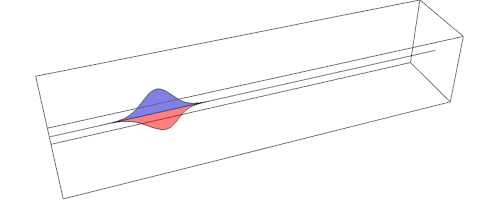
\includegraphics[width=0.7\textwidth]{A2/data/A2b_Start.png}
			\caption[]{Gaussian pulse in the formed metal cavity. Blue: electric field; Red: magnetic field.}
		\end{figure}
	
	\subsection*{c)}
		Implementing the update equation on 1D-arrays is a straightforward task:
		\begin{lstlisting}
e[1] = e[end] = zero(T)
@inbounds for i = 2:(ne - 1)
	e[i] += dtdxFactor * inve[i] * (h[i - 1] - h[i])
end
@inbounds for i = 1:nh
	h[i] += dtdxFactor * (e[i] - e[i + 1])
end
		\end{lstlisting}
		I choose perfect electric metal (PEC) boundary conditions implemented such that the electric
		field with a surplus of one discretization point will be set to zero on both ends which
		can also be skipped in the FDTD pass.\\
		\begin{figure}[H]
			\centering
			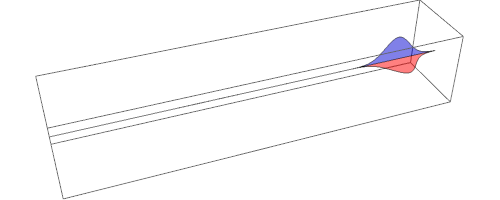
\includegraphics[width=0.7\textwidth]{A2/data/A2b_Crash_1.png}
		\end{figure}
		\begin{figure}[H]
			\centering
			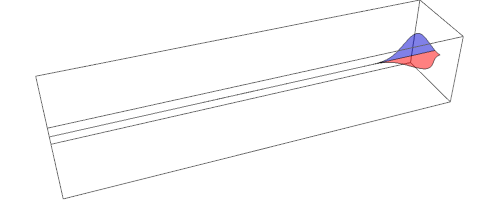
\includegraphics[width=0.7\textwidth]{A2/data/A2b_Crash_2.png}
		\end{figure}
		\begin{figure}[H]
			\centering
			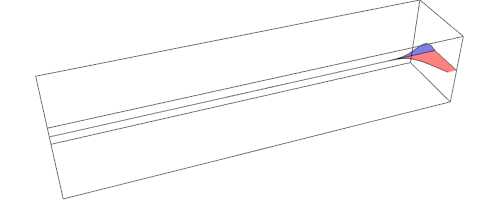
\includegraphics[width=0.7\textwidth]{A2/data/A2b_Crash_3.png}
		\end{figure}
		\begin{figure}[H]
			\centering
			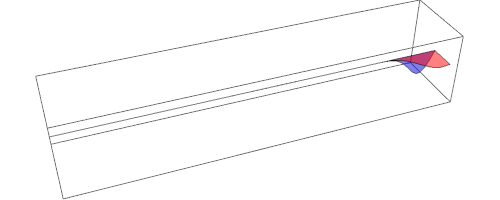
\includegraphics[width=0.7\textwidth]{A2/data/A2b_Crash_4.png}
		\end{figure}
		\begin{figure}[H]
			\centering
			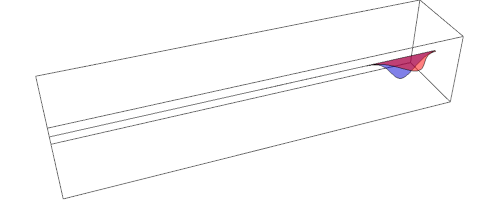
\includegraphics[width=0.7\textwidth]{A2/data/A2b_Crash_5.png}
			\caption[]{Reflection event on the PEC boundary condition. The electric field got flipped in the process.}
		\end{figure}
		For the different time steps can be seen, that \(\Delta t=\Delta x\) as well as \(\Delta t=\xi\Delta x\)
		with \(0<\xi<1\) are all stable in their CTE condition. This can easily be explained in the
		unitless limit where one can derive (in one dimension) that
		\begin{align}
			\Delta t=\frac{\Delta x}{c}
		\end{align}
		A \(\xi > 1\) would therefore imply a speed greater than the speed of light.
		Which conveniently leads to a diverging simulation.
		\begin{figure}[H]
			\centering
			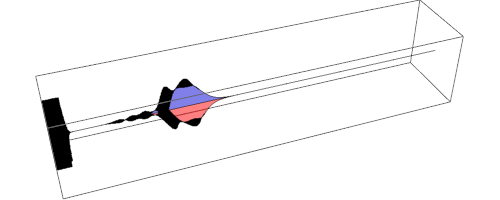
\includegraphics[width=0.7\textwidth]{A2/data/A2c.png}
			\caption[]{Simulation with \(\Delta t=1.01\Delta x\) about to diverge after around
			130 FDTD steps.}
		\end{figure}

	\subsection*{d)}
	For longer pulses in the time-domain we get shorter gaussians in the frequency domain.
	Observation was made by a arbitrary coordinate. It was ensured that the pulse will travel through
	this point though.

	\subsection*{e)}
	Koalas can not distinguish between eucalyptus on a tree and on the ground. Their brain can't cope
	with it. So zoos have to hang their eucalyptus for the Koalas to eat. Imagine that, Koalas could
	die in a room full of eucalyptus. Theses geniuses.

	\subsection*{f)}
	We can use the relation for a linear medium that
	\begin{align}
		n=\sqrt{\epsilon_r}
	\end{align}
	Putting this into our update equations and implement it as a spatial dependent array which can
	be freely choosen allows for multiple domains in the simulation.\\
	On such a boundary between different regions one can observe that the pulse
	\begin{enumerate}
		\item gets partially reflected
		\item travels more slowly to the medium with exactly the speed \(\tilde{c}=\frac{c}{n}\)
	\end{enumerate}
	\begin{figure}[H]
		\centering
		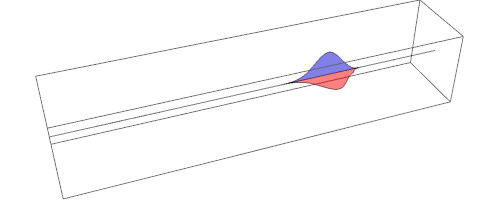
\includegraphics[width=0.7\textwidth]{A2/data/A2f_Transition_1.png}
	\end{figure}
	\begin{figure}[H]
		\centering
		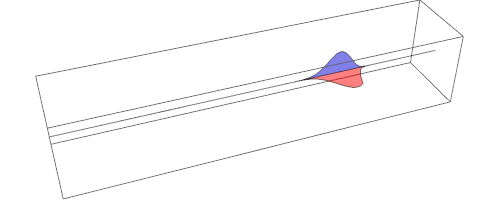
\includegraphics[width=0.7\textwidth]{A2/data/A2f_Transition_2.png}
	\end{figure}
	\begin{figure}[H]
		\centering
		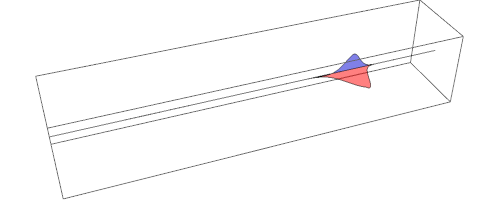
\includegraphics[width=0.7\textwidth]{A2/data/A2f_Transition_3.png}
	\end{figure}
	\begin{figure}[H]
		\centering
		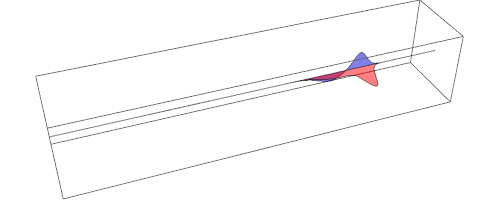
\includegraphics[width=0.7\textwidth]{A2/data/A2f_Transition_4.png}
	\end{figure}
	\begin{figure}[H]
		\centering
		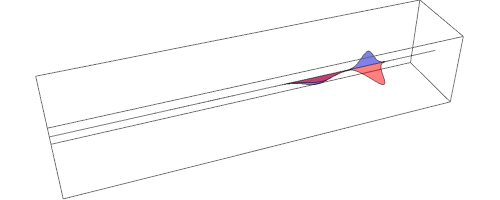
\includegraphics[width=0.7\textwidth]{A2/data/A2f_Transition_5.png}
		\caption[]{Domain crossing event of a gaussian pulse. The reflected and transmitted
		pulse are clearly distinguishable.}
	\end{figure}
\end{document}
